\documentclass{article}%
\usepackage[T1]{fontenc}%
\usepackage[utf8]{inputenc}%
\usepackage{lmodern}%
\usepackage{textcomp}%
\usepackage{lastpage}%
\usepackage{authblk}%
\usepackage{graphicx}%
%
\title{The Retromer Complex Is Required for Rhodopsin Recycling and Its Loss Leads to Photoreceptor Degeneration}%
\author{Linda Moody}%
\affil{Neurophysiology Laboratory, Department of Pharmacology and Experimental Neuroscience, University of Nebraska Medical Center, Omaha, Nebraska, United States of America}%
\date{01{-}01{-}2014}%
%
\begin{document}%
\normalsize%
\maketitle%
\section{Abstract}%
\label{sec:Abstract}%
Hepatitis B infection is the most common killer in the United States. There are about 900,000 new cases diagnosed each year in the United States, and about 75,000 people die from the disease each year.\newline%
One of the most common causes of infection is through blood transfusions and other organ transplantation.\newline%
The most prominent cause of liver damage is liver cancer. More than half the patients dying of liver cancer will develop liver cirrhosis, which is an abnormal scarring.\newline%
Pathological Impact: Pathological Impact of Hepatitis B Virus Surface Protein\newline%
The new research found a gene called epidermolysis bullosa, or EB, that leads to the low{-}density lipoprotein receptor (LDLR) in the liver, which has long been linked to the deficiency of hemoglobin.\newline%
The study was published today in the Proceedings of the National Academy of Sciences.\newline%
Researchers say that having epidermolysis bullosa can also be directly related to the genetic basis of cystic fibrosis, which afflicts about 10,000 children in the United States.

%
\subsection{Image Analysis}%
\label{subsec:ImageAnalysis}%


\begin{figure}[h!]%
\centering%
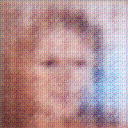
\includegraphics[width=150px]{500_fake_images/samples_5_117.png}%
\caption{A Man With A Beard Wearing A Red Tie}%
\end{figure}

%
\end{document}